%!TEX root = ../../Main.tex
\graphicspath{{Chapters/Opgave1/}}
%-------------------------------------------------------------------------------

\chapter{Signal generation}
Via det vedlagte MATLAB-kode ”CrosscoreHelper” har vi genereret en fil, som indeholder et ”chirp”, altså et frekvenssweep. Ved test af forskellige frekvenser fandt vi ud af at den højtaler vi brugt ikke reagerede så godt på lave frekvenser. Vi har derfor lavet et sweep mellem 2000Hz og 3500Hz.
Det vil ikke være fordelagtigt at bruge en ren sinus-tone, da periodiske signaler giver en tilsvarende periodisk krydskorrelation som vist på billedet nedenfor \autoref{fig:Sinus}

\begin{figure}[H]
\centering
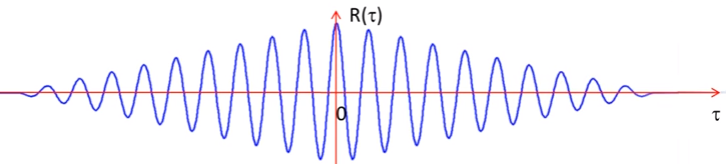
\includegraphics[width = 300pt]{Img/Sinus.PNG}
\caption{Krydskorrelation ved periodisk signal}
\label{fig:Sinus}
\end{figure}

Problemet med dette er at der ikke skal meget støj til på signalet, før det vil være svært at vurdere hvilket af de mange peaks der er det største. Krydskorrelation af et ikke-periodisk signal vil derimod kun have et enkelt peak, hvilket gør det nemmere at estimere tidsforskellen.
Det vil desuden være fordelagtigt at bruge et længere signal, da krydskorrelationen i så fald vil være mindre sårbar overfor støj. Hvis man ved at overdrive siger at man har et signal på ét enkelt sample vil krydskorrelationen give peaks alle steder hvor det modtagne støjsignal har samme værdi som vores signal. Jo flere samples der er i vores signal, des mindre lighed vil der dog være imellem tilfældig støj og vores signal. Der vil dog være andre faktorer man skal have i mente, så som hukommelse i ens system, og tiden det tager at udregne krydskorrelationen. I vores tilfælde var vi begrænset af at vi på Blackfin’en ikke kunne benytte et signal, der var større en 20kB.

Afstanden som ét sample svarer til kan findes ud fra Blackfin’ens sampletid og lydens hastighed i det givne miljø.

\begin{figure}[H]
\centering
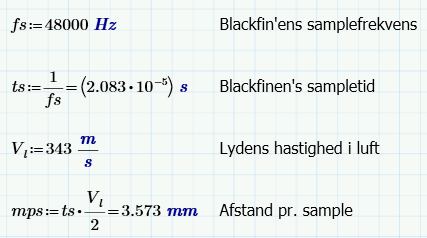
\includegraphics[width = 300pt]{Img/UdregningSample.PNG}
\caption{Udregninger for afstand pr sample}
\label{fig:UdregningSample}
\end{figure}

